\chapter{ Fermionic States, its characterisation and the connection with Coding theory.}
Up to this point we provided a detailed explanation of how in quantum mechanical description, reaching equilibrium emerges as a consequence of the structure of quantum mechanics. Even more, we stated that in the case we deal with states which its eigenenergies are close to each other, typicality will also provide us an answer of how this kind of states will reach equilibrium. As we would like to illustrate this phenomena occur, we focus our study in the fermionic case. In this Chapter we are Going to provide a background to understand how fermionic states are usually treated and why we choose to work with them. More specifically, we provide the overview of solvable fermionic systems, its connection to Majorana fermions and Gaussian states, the formalism of Grassmann for anticommuting variables, and the link between all the formalism for fermions and coding theory.\\
\section{Overview}
In many areas of physics one has to deal with solving quantum many body problems, which is often a computationally difficult if not impossible task. However, the cases which can be annalitically solved are very well known, and some assumptions have to be taken into account. In spite of this considerations it has been found that a wide class of complicated Hamiltonians with many-body interactions can be often be mapped onto Hamiltonians that are quadratic in annihilation and creation operators and have the generic form \cite{botero_bcs-like_2004}

\begin{equation}
\hat{H}=\sum_{i j} C_{i j} \hat{a}_{i}^{\dagger} \hat{a}_{j}+\sum_{i j}\left(A_{i j} \hat{a}_{i}^{\dagger}\hat{a}_{j}^{\dagger}+\mathrm{h.c.}\right),
\label{CH2:QuadraticHamiltonian}
\end{equation}

where $i,j$ run from $1$ to the number of modes in the system ($N$) and $\hat{a}_i$, $\hat{a}^{\dagger}_i$ are Fermionic annihilation and creation operators which satisfy the canonical anti-commutation relations (CAR)\cite{fradkin_field_1997}

\begin{equation}
\left\{\hat{a}_{k}, \hat{a}_{l}\right\}=\left\{\hat{a}_{k}^{\dagger}, \hat{a}_{l}^{\dagger}\right\}=0, \quad\left\{\hat{a}_{k}, \hat{a}_{l}^{\dagger}\right\}=\delta_{k l}.
\label{CH2:Anticommutation}
\end{equation}

A convenience when working with these kind of Hamiltonians is that can be diagonalized via a Bogoliubov- Valantin transformations transformation (i.e., canonical transformations), which maps Fermionic creation and annihilation operators on the creation and annihilation operators of non-interacting quasi-particles\cite{berezin_method_1966,bogoljubov_new_1958}. Explicitly the transformation looks like

\begin{equation}
\begin{array}{c}
\hat{a}_{i} \mapsto \gamma_{i} \hat{q}_{i}+\kappa_{i} \hat{q}_{i}^{\dagger}, \\
\hat{a}_{i}^{\dagger} \mapsto \bar{\gamma}_{i} \hat{q}_{i}^{\dagger}+\bar{\kappa}_{i} \hat{q}_{i}.
\end{array}
\label{CH2:Bogoliuvov}
\end{equation}

where $\gamma_i , \kappa_i$ are complex numbers such that preserves the canonical anti-commutation relations given by \eqref{CH2:Anticommutation} for $\hat{q}$, $\hat{q}^{\dagger}$\footnote{This relation can also be expresses as a condition over $\gamma_i , \kappa_i$,
\[ \gamma_i ^2+ \kappa_i^2 = 1,\]
and 
\[\left\{\hat{q}_{k}, \hat{q}_{l}\right\}=\left\{\hat{q}_{k}^{\dagger}, \hat{q}_{l}^{\dagger}\right\}=0, \quad\left\{\hat{q}_{k}, \hat{q}_{l}^{\dagger}\right\}=\delta_{k l}.\]
 }.
\\
Many relevant physics models are diagonalizable via a Bogoliubov-Valantin transformations, some examples are the Hubbard model, BCS theory of superconductivity in the mean field or Hartree-Fock approximation, and certain solvable spin-chain models (After a Jordan-Wigner transformation) \cite{fradkin_field_1997}. As we will later explain, an important feature about the class of Hamiltonians described by \eqref{CH2:QuadraticHamiltonian}, if not the most important for the purpose of this project,  is that not only the ground state (quasi-particle vacuum)  but all eigenstates describing a excitation  in a set of quasi-particles, belong to the class of so-called Fermionic Gaussian states\cite{botero_bcs-like_2004}. What is important about this class of states is that are fully characterized by second order correlations, because all the higher moments factorize. This result is very well known and as Wick theorem \cite{westwanski_general_1973,molinari_notes_2017}.
\section{Majorana Fermions}
Majorara fermions are fermions such that they are their own antiparticle. In the frame of condensed matter Majorana Fermions (quasi-particles) can be interpreted as a superposition of a electron state and a hole \cite{leijnse_introduction_2012}.
\\
The formalism of Majorana fermions or Majorana modes of the system (with $N$ modes) can be introduce with the operators
\begin{equation}
\hat{c}_{2j-1}=\hat{a}_{j}^{\dagger}+\hat{a}_{j}, \quad \hat{c}_{2j}=(-i)\left(a_{j}^{\dagger}-a_{j}\right).
\label{CH2:majorana}
\end{equation}
In which case its canonical anti-commutation relations (CAR) take the form
\begin{equation}
\left\{\hat{c}_{k},\hat{c}_{l}\right\}=2 \delta_{k l}.
\label{CH2:CAR_majorana}
\end{equation}

The anti-commutation relations is seen to be a consequence of an $\mathbb{R}^{2N}$ Clifford algebra\footnote{By inspection of \eqref{CH2:CAR_majorana} we see that  any linear transformation of the form $\tilde{\gamma}_{\alpha} = O_{\alpha\beta}\gamma_{\beta}$ where $O\in SO(2N)$, the special orthogonal group in $2N$  dimensions}. Transformation in between Fermionic and Majorana operators is achieved by matrix of the block form
\begin{equation}
\Omega=\left(\begin{array}{cc}
\mathbb{I} & \mathbb{I} \\
i \mathbb{I} & -i \mathbb{I}
\end{array}\right),
\end{equation}

and then the map from Fermionic ($\vec{\hat{a}}^{T} = (\hat{a}_1,\ldots,\hat{a}_1^{\dagger},\ldots)$) and Majorana ($\vec{\hat{c}}^{T} = (\hat{c}_1,\ldots,\hat{c}_1^{\dagger},\ldots)$) operators is written as $\Omega\vec{\hat{a}}=\vec{\hat{c}}$.
\\
By changing from Fermionic operators to Majorana operators is possible, and convenient, to define de Fermionic covariance matrix which as we mentioned before, fully characterise Gaussians states\footnote{In comparison to its boson counterpart the fermion Gaussian states have the property that correlation functions for the creation/annihilation operators are completely determined by the two-point functions according to Wick’s theorem \cite{westwanski_general_1973}, and moreover,  since this property is extensible to correlation function pertaining to a reduced subset of the modes, it follows that any partial (reduced) density matrix obtained from $\rho$ remains Gaussian.}.

\section{Fermionic Covariance matrix }
A system of $N$ fermion modes, described by a set of creation and annihilation operators $\hat{a}^{\dagger}, \hat{a}$  and satisfying the  canonical anti-commutations relations in \eqref{CH2:Anticommutation}, is Gaussian if for such system any state $\rho$ can be written as  \cite{cheong_many-body_2003}

\begin{equation}
\rho=\bigotimes_{k=1}^{N} \tilde{\rho}_{k}, \quad \tilde{\rho}_{k}=\frac{1}{2}\left(1-\lambda_{i}\left[\tilde{a}_{i}^{\dagger}, \tilde{a}_{i}\right]\right),
\label{CH2:rho_gaussiano_no_exp}
\end{equation}

for a certain choice of mode basis $\tilde{a}=u_{i}^{j}\hat{a}_{j} + v_{i}^{j}\hat{a}_{j}^{\dagger}$, and with $|\lambda_i|\leq 1$, where the equality holds for pure states. Equivalently, as mentioned before, Gaussian States are fully characterized by their second moments, so an equivalent form of writing $\rho$ is
\begin{equation}
\rho= \frac{1}{Z}\cdot \exp \left[-\frac{i}{4} \hat{c}^{T} G \hat{c}\right],
\label{CH2:rho_gaussiano_exp}
\end{equation}
with $\hat{c} = (\hat{c}_1,\hat{c}_2,\ldots,\hat{c}_{2N})$, the vector of Majorana operators \eqref{CH2:majorana}, $Z$ a normalization constant and $G$ real anti-symmetric $2N\times 2N$ matrix. 
\\
Since $G$ is a skew-symmetric matrix, it can always be brought to the block diagonal form 
\begin{equation}
O G O^{T}=\bigoplus_{i=1}^{N}\left(\begin{array}{cc}
0 & -\beta_{j} \\
\beta_{j} & 0
\end{array}\right) \quad \text { with } \quad O \in \mathrm{SO}(2 \mathrm{N}),
\label{CH2:MatrixG_Williamson}
\end{equation}
by a special orthogonal matrix $O\in SO(2N)$ where the $\beta_{j}$ are called the Williamson eigenvalues of the matrix $G$. 
From equation \eqref{CH2:rho_gaussiano_exp} it is clear that Gaussian states have an interpretation as thermal (Gibbs) states corresponding to a Hamiltonian of the form
\begin{equation}
\hat{H}=\frac{i}{4} \hat{c}^{T}G\hat{c}= \frac{i}{4} \sum_{k>l}G_{kl}\left[\hat{c}_{k},\hat{c}_{l}\right]
\label{CH2:Hamiltonian_majorana}
\end{equation}

and \eqref{CH2:MatrixG_Williamson} shows that every Gaussian state has a normal mode decomposition in terms of $N$ single mode ``thermal states'' of the form \eqref{CH2:rho_gaussiano_no_exp} ($\sim \text{exp}(-\beta \hat{a}^{\dagger}\hat{a})$)\cite{kraus_pairing_2009}. From this is clear, that the state can be fully determined by the expectation values of quadratic operators $(\hat{a}_i^{(\dagger)}\hat{a}_j^{(\dagger)}$ and  $\hat{a}^{\dagger}_i\hat{a}_j)$. So collecting these expectation values in a real and skew-symmetric covariance matrix $\Gamma$ which is defined via
\begin{equation}
\Gamma_{k l}=\frac{i}{2} \operatorname{tr}\left(\rho\left[c_{k}, c_{l}\right]\right).
\label{CH2:Cov_matrix_elements}
\end{equation}
We will be able to bring this anti-symmetric matrix to its block diagonal form, via a canonical transformation.
\begin{equation}
\tilde{\Gamma} = O \Gamma O^{T}=\bigoplus_{i=1}^{M}\left(\begin{array}{cc}
0 & \lambda_{i} \\
-\lambda_{i} & 0
\end{array}\right),
\label{CH2:Williamson_Cov_fermionic_matrix}
\end{equation}
with $\lambda_i\geq 0$ the Williamson eigenvalues.\\
In terms of the creation/annihilation operators obtained from the transformed $\tilde{c}=O\hat{c}$, the Gaussian state $\rho$ takes the form \eqref{CH2:rho_gaussiano_exp} with $\tilde{\Gamma}$ as its Fermionic covariance matrix. It is easy to see that the relation between $G$ and $\Gamma$ is given by $\lambda_{i} = \tanh{\left(\beta_{i}/2\right)}$, for $i=1,2,\ldots,N$\cite{kraus_pairing_2009}. 
\newline
The equivalence between the special orthogonal group in $2N$ dimensions ($SO(2N)$) and the Fermionic Gaussian states, drives to an interesting  property about states describing multi-particles excitations. If $\ket{\textit{vacuum}}$ is the ground state of some Hamiltonian, with annihilation operators $\hat{a}_{i}$ in a given quasi-particle basis, then $\hat{a}_{i}^{\dagger}\ket{\textit{vacuum}} = \hat{c}_{2i}\ket{\textit{vacuum}}$. Meaning that any multi-particle state of this kind is obtained from some transformation (that preserves the canonical anti-commutation relations) of the ground state $\ket{\textit{vacuum}}$, remains Gaussian. In other words, Gaussian states are preserved under any unitary transformation that preserves anti-commutation relations.
\newline 
The fact that all eigenstates of the Hamiltonian in \eqref{CH2:QuadraticHamiltonian} are Gaussian as well as the extension of this property to a reduced subset of the modes, is quite important since a big part of this work is focused on the study of the Fermionic covariance matrix of the $XY$ model.\\
Up to this point we have talked about some generalities about the quadratic Hamiltonians and how these can be brought to its diagonal form to be analytically solved. However, one may wonder how is this connected to some observables, if the Fermionic covariance matrix has something to do in the observables. The answer to these questions will be boarded in the next section in which we will provide the formalism needed to compute observables over anti-commuting variables as well as the differences we will have between bosons and fermions.
\section{Grassmann Approach}
Fermions are one kind of fundamental particles which can be used to represent quantum information, being one posibility to do quantum computation. From Knill, Laflamme and Milburn\cite{knill_scheme_2001} work, we know that it is possible to provide an universal set of operations for quantum computation by just using passive linear objects. Right after this discovery, Terhal, DiVincenzo\cite{terhal_classical_2002} and knill\cite{knill_fermionic_2001} provided a description of the computational capability for Fermionic linear optics (FLO)\footnote{Whenever we are referring to this term, it basically has in consideration a system consisting of non-interacting electrons in a controllable external potential and a detector that measures projectively occupation numbers of single-electron modes.}. These results show that FLO is not a promising way to do quantum computation, since it can be efficiently simulated by classical means, on the other hand, this provides a very interesting tool to study general properties quantum channels for quantum communication.\\
When working with fermions one could think, weather or not is possible to use the same formalisms than the ones used when working with bosons\footnote{By this we mean that it could be also written in its correspond operators of annihilation and creation $\hat{a}^{\dagger}$,$\hat{a}$\cite{noauthor_density_2007}}, and as expected many features between them are shared. More specifically, in the case of FLO, it shares most of the features with a limited version of photon linear optics, where mostly Gaussian states appears\cite{knill_scheme_2001}\footnote{the main reason for this is that a set of states that can be achieved by FLO operations starting from the Fock vacuum is a set of Fermionic Gaussian states, just as the case of its bosonic counterpart.}.\\
It is worth mentioning that some of the results in here are quite general and can be used even beyond the scope of our work.

%In Quantum Optics the most common states we work with, are the so-called coherent states,  these states are of great importance since these states turned out to be a proper basis for describing all states of electromagnetic field, are also well known for its intrinsic property that the particle number of such states is indefinite, while the phase is determined exactly\cite{QuantumOptics_wolfgang}, therefore these states can be seen as the counter part of the Fock states\footnote{States that belong to the Fock space have the property that their particle number is well defined but not its phase.}\\When working with fermions one could think if weather or not is possible to use the same formalisms than the ones used when working with bosons\footnote{With its operators of annihilation and creation $\hat{a}^{\dagger}$,$\hat{a}$}\cite{noauthor_density_2007}. The study of Fermionic system is know as Fermionic Linear Optics (FLO). FLO shares many features with a limited version of photon linear optics, where mostly Gaussian states appears\cite{knill_scheme_2001}. The main reason for this is that non-interacting fermion, as well as bosons, are described byin the Lagrangian representation  by Gaussian integrals over anti-commutating (commutating) variables\cite{bravyi_lagrangian_2004}. The states achievable with FLO belong to a closure of a low dimensional Lie group\footnote{Growing only quadratically with the number of modes}. The elements of this Lie group are known as  Gaussian operators \cite{knill_fermionic_2001}, which are the states we mentioned in the latter section and we defined as operators that can be represented as an exponential of another operator which is quadratic in the creation/annihilation operators\footnote{Even though this definition is not valid in cases when the operator does not have full rank, the definition we use here fits for the purpose of this work}.\\

\subsection{Fermionic Linear Optics}
In order provide a more specific description of FLO, we start by defining $N$ abstract Fermionic modes which can be defined by creation $\hat{a}_j$ and annihilation $\hat{a}_j^{\dagger}$, $j=1,\ldots,N$, satisfying \eqref{CH2:Anticommutation}. As mentioned above, any state of the system can be generated from the vacuum state $\ket{\textit{vacuum}}$ of the Fock basis, which we define as
\begin{equation}
\ket{N_1,\ldots,N_{N}} = \left(\hat{a}_{1}^{\dagger}\right)^{N_{1}} \cdots\left(\hat{a}_{n}^{\dagger}\right)^{N_{n}}\left|\textit{vacuum}\right\rangle,
\label{CH2:Fock_Space}
\end{equation}
with $N_i\in \{0,1\}$. We have then that any sequence $\{N_i\}$ can be understood as a Fermionic state which comes from a superposition of the Fock basis.\\
When working with FLO, quadratic Hamiltonians govern the dynamics, in which terms associated with individual energy modes, tunneling and bulk dynamics are included. The structure of these Hamiltonians is what allow us conveniently work with operators which generate the \textit{Clifford} algebra ($\mathcal{C}_{2N}$), described in \eqref{CH2:CAR_majorana}. So we will have that any arbitrary operator $X\in \mathcal{C}_{2N}$ will be written as a polynomial in the operators $\{\hat{c}_a\}$ as
\begin{equation}
X=\alpha \hat{I}+\sum_{p=1}^{2 n} \sum_{1 \leq a_{1}<\cdots<a_{p} \leq 2 n} \alpha_{a_{1}, \ldots, a_{p}} \hat{c}_{a_{1}} \cdots \hat{c}_{a_{p}},
\label{CH2:operators_in_clifford}
\end{equation}

with $\alpha=2^{-n} \operatorname{Tr}(X)$. Particularly for the Hamiltonian operator we have that
\begin{equation}
H=\frac{i}{4} \sum_{a, b=1}^{2 N} H_{a b} \hat{c}_{a} \hat{c}_{b},
\label{CH2:Hamiltonian_in_CLifford}
\end{equation}

with $\{H_{a b}\}$ an anti-symmetric $2N\times 2N$ matrix.\\
We may think that when working with fermions could be the same as working with bosons by changing commutators with anti-commutators and changing to a fine algebra. However, this is not the case, as we will show in the next section observables have to be computed by using the corresponding calculus for fermionic systems.

%However, instead of working with the operator of creation/annihilation we instead work with operators described previously in \eqref{CH2:majorana}, which generate the \textit{Clifford} algebra ($\mathcal{C}_{2N}$) described in \eqref{CH2:CAR_majorana}. Thus Hamiltonians of the form \eqref{CH2:QuadraticHamiltonian} can be brought to the form of \eqref{CH2:Hamiltonian_majorana}. Something to stress is the fact that unitary elements of FLO constitute a group of \textit{canonical transformations} $G_{c}\subset U(2^{N})$\footnote{This can be translated as $V\in G_{c}$ if and only if $V= \exp(i\hat{H})$, with $\hat{H}$ from \eqref{CH2:Hamiltonian_majorana}}, making then see the action of a canonical transformation $V\in G_c$ on the operators $\{\hat{c}_a\}$ as a rotation $R\in SO(2N)$.\\
%When working with FLO we could naively think the formulation should be as if we work with bosons, however, this is not the case, certainly, we can make an analogue formulation as the one on bosons. The first problem we deal is that unitary elements of FLO do not preserve the total number of particles, and we do not have a preferred vacuum state, and neither we have a preferred normal ordering of Fermionic operators. Secondly we often would like to treat both pure and mixed states on equal footing\cite{francesco_conformal_1997}. To address these problems we are going show a brief outline of the anti-commutating variables formalism.


\subsection{Grassmann Calculus}
There are a lot of results from the earlier seventies which describe techniques to study systems with infinite number of fermionic modes \cite{soper_construction_1978}, nonetheless, the formalism we are going to present here is a specific case where  a finite number of modes is considered, and consist in a customization of the Lagrangian representation for infinite number of Fermionic modes, presented in \cite{bravyi_classical_2005}. 
Consider $\theta_{1},\ldots,\theta_N$ span a N-dimensional complex linear space $\mathbb{C}^{N}$. From the anti-commutation relation we get that for $\theta_{1},\ldots,\theta_N$,
\begin{equation}
\theta_{a}^{2}=0 \quad \text { and } \quad \theta_{a} \theta_{b}+\theta_{b} \theta_{a}=0,
\label{CH2:Grassmann_anticommutation}
\end{equation}

so it is clear that the most general function we can built over the Grassmann algebra with complex coefficients $\mathcal{G}_{N}$ is  a polynomial of $\theta$'s
\begin{equation}
f(\theta)=\alpha+\sum_{p=1}^{n} \sum_{1 \leq a_{1}<\cdots<a_{p} \leq N} \alpha_{a_{1}, \ldots, a_{p}} \theta_{a_{1}} \cdots \theta_{a_{p}},
\label{CH2:Grassmann_function}
\end{equation}
where the coefficients $\alpha_{*}$ are complex numbers. A polynomial $f(\theta)$ will be called \textit{even} if it involves only even powers of $\theta$, nonetheless something to stress is that even elements constitute the center of the Grassmann algebra.\\
It is possible to differentiate functions of Grassmann variables. A partial derivative over $\theta_{a}$ is a linear operator from $\mathcal{G}_{N}$ to $ \mathcal{G}_{N}$, which is defined by
\begin{equation}
\frac{\partial}{\partial \theta_{a}} 1=0, \quad \frac{\partial}{\partial \theta_{a}} \theta_{b}=\delta_{a b},
\label{CH2:Grassmann_diferential}
\end{equation}
and Liebniz's rule
\begin{equation}
\frac{\partial}{\partial \theta_{a}}\left(\theta_{b} f(\theta)\right)=\delta_{a b} f(\theta)-\theta_{b} \frac{\partial}{\partial \theta_{a}} f(\theta).
\label{CH2:Grassmann_diferential_liebniz}
\end{equation}
The equality \eqref{CH2:Grassmann_diferential_liebniz} implies that 
\begin{equation}
\left\{\frac{\partial}{\partial \theta_{a}}, \frac{\partial}{\partial \theta_{b}}\right\}=0.
\label{CH2:Grassmann_partial_derivative_anticommutation}
\end{equation}
Since a derivative $\frac{\partial}{\partial\theta_{a}}f(\theta)$ does not depend upon variable $\theta_{a}$, it is sometimes convenient to think about differentiation as a linear operator mapping $\mathcal{G}_{n}$ into $\mathcal{G}_{n-1}$. Such operator is called integration and is denoted as\cite{bravyi_lagrangian_2004} \footnote{Here we will use a compact notation \[\int \mathrm{D} \theta \equiv \int d \theta_{n} \cdots \int d \theta_{2} \int d \theta_{1},\] and the order is chosen such that \[\int D\theta\ \theta_1\cdots\theta_n = 1\].
}
\begin{equation}
\int d \theta_{a} \equiv \frac{\partial}{\partial \theta_{a}}: \mathcal{G}_{n} \rightarrow \mathcal{G}_{n-1}.
\label{CH2:Grassmann_Integration_relation}
\end{equation}

From equation \eqref{CH2:Grassmann_partial_derivative_anticommutation}  we have that
\begin{equation}
\int \mathrm{D} \theta \frac{\partial}{\partial \theta_{a}} f(\theta)=0,
\end{equation}
this equation combined with \eqref{CH2:Grassmann_diferential_liebniz} give us the anti-commuting version of integration by parts.
\newline
With these properties we show the main equation that will help us calculate what is need for the purpose of this work.
\newline
\textit{For a vectors of Grassmann variables  $\vec{\theta}$, $\vec{\eta}$ and complex anti-symmetric matrix $M$ we have}

\begin{equation}
\int \mathrm{D} \theta \exp \left(\frac{i}{2} \theta^{T} M \theta\right)=i^{n} \operatorname{Pf}(M),
\label{CH2:Grassman_property_1}
\end{equation}
and
\begin{equation}
\int \mathrm{D} \theta \exp \left(\eta^{T} \theta+\frac{i}{2} \theta^{T} M \theta\right)= i^{n} \operatorname{Pf}(M)  \cdot \exp \left(-\frac{i}{2} \eta^{T} M^{-1} \eta\right).
\label{CH2:Grassman_property_2}
\end{equation}
In these formulas $\operatorname{Pf}(N)$ is the Pfaffian of a complex antisymmetric matrix $N$ defined as  anti-symmetrized product $\mathcal{A}(N_{1,2}N_{3,4}\cdots N_{2n-1,2n})$ that is
\begin{equation}
\operatorname{Pf}(N)=\frac{1}{2^{n} n !} \sum_{\sigma \in S_{2 n}} \operatorname{sgn}(\sigma) N_{\sigma_{1}, \sigma_{2}} \cdots N_{\sigma_{2 n-1} \sigma_{2 n}}
\label{CH2:Grassmann_Pfaffian}
\end{equation}
\subsection{Gaussian States}

For this part we are going to introduce in a formal way the states we have been talking about in at the beginning of this chapter. Informally we can say that any Gaussian operator can be represented as an exponent of another operator which is quadratic in creation/annihilation operators. When considering an operator $X\in\mathcal{C}_{2N}$ It is natural to assign a polynomial $\omega(X,\theta)\in \mathcal{G}_{2N}$ of $2N$ Grassmann variables defined by
%Here we introduce the Grassmann version of the covariance matrix approach showed in \cite{bravyi_lagrangian_2004}. It turns out that the connection between these two approaches is the map assigning the Grassmann variable to each Majorana operator.
%\newline
%Consider $X$ to be a linear operator on the Clifford algebra $\mathcal{C}_{2n}$ that is generated by Majorana operators given in \eqref{CH2:majorana}fulfilling the CAR in \eqref{CH2:CAR_majorana}. One can naturally assign a polynomial in Grassmann variables via

\begin{equation}
\omega\left(\hat{c}_{p} \hat{c}_{q} \cdots \hat{c}_{r}, \theta\right)=\theta_{p} \theta_{q} \cdots \theta_{r}, \quad \omega(\hat{\mathbb{I}}, \theta)=1,
\label{CH2:Gaussian_majorana_map_majorana}
\end{equation}
where this definition comes from the general functions in the Grassmann algebra described in \eqref{CH2:Grassmann_function}.
%\footnote{This definition extends by linearity to an arbitrary $X\in \mathcal{C}_{2n}$. It should be enphasized that $\omega$ is just an isomorphism of linear spaces and it has nothing to do with multiplication in the algebras $\mathcal{C}_{2n}$ and $\mathcal{G}_{2n}$}.
\newline
To illustrate what how this map can be done, consider as an example the projector $\hat{a}_1\hat{a}_1^{\dagger}$, which its action is nothing but to project into a state where the first mode is empy. For this precise case we have that the map to Grassmann variables will look as

%Then we define a state in terms of Gaussianity of its Grassmann representation. A quantum state of $n$ fermionic modes is Gaussian if and only if its operator  $\rho\in\mathcal{C}_{2n}$ has a Gaussian Grassmann representation given by 
\begin{equation}
\omega(\hat{a}_1\hat{a}_1^{\dagger}, \theta)=\frac{1}{2} \left(\mathbb{I}+ i \theta_1\theta_2\right) =\frac{1}{2}  \exp \left(i \theta_1\theta_2\right),
\label{CH2:Gaussian_Grassmann}
\end{equation}
where all exponents were defined by a Taylor series.\\
\newline
For any two operators $X,Y\in \mathcal{C}_{2N}$ one can compute the trace by just using a simple formula,
\begin{equation}
\operatorname{Tr}(X Y)=(-2)^{N} \int D \theta D \mu e^{\theta^{T} \mu} \omega(X, \theta) \omega(Y, \mu),
\label{CH2:Trace_grassmann_operators}
\end{equation}
 which can be directly verified.
It is also easy to see that canonical transformations of an operator $X\in\mathcal{C}_{2N}$ are equivalent to an orthogonal change of basis in the space of the Grassmann variables, this is
\begin{equation}
\omega\left(V X V^{\dagger}, \theta\right)=\omega(X, \eta), \quad \eta_{a}=\sum_{b=1}^{2 n} R_{a b} \theta_{b}.
\label{CH2:Transformations_in_Grassmann_Variables}
\end{equation}
So we will define  a Gaussian states of N Fermionic modes as via its density operator $\rho\in\mathcal{C}_{2N}$. We say that a state is Gaussian in  $\mathcal{C}_{2N}$ \textit{iff} its Grassmann representation is as well Gaussian
\begin{equation}
\omega(\rho, \theta)=\frac{1}{2^{n}} \exp \left(\frac{i}{2} \theta^{T} M \theta\right),
\end{equation}
for some $2N\times 2N$ antisymmetric matrix $M$. The matrix $M$ is defined as 
\begin{equation}
M_{a b}=\frac{i}{2} \operatorname{Tr}\left(\rho\left[\hat{c}_{a}, \hat{c}_{b}\right]\right)=\left\{\begin{aligned}
\operatorname{Tr}\left(\rho i \hat{c}_{a} \hat{c}_{b}\right) & \text { for } a \neq b \\
0 & \text { for } a=b
\end{aligned}\right. ,
\end{equation}
which is nothing but the covariance Fermionic matrix defined in \eqref{CH2:Cov_matrix_elements}, meaning that it can be brought to its Williamson form to get its eigenvalues.\\
\newline
Therefore the connection between the Grassmann formalism for Gaussian states and the Fermionic covariance matrix described at the beginning of the chapter, is easily understood by simply assigning the correspondent covariant matrix to the states we work with. Nonetheless, one could be wondering how is this formalism connect to the error correcting code theory. In the next section we will provide a little historical background of how this theory was done and how one can think states of fermions as binary codes. More specifically we will provide the necessary background to link the theory of correcting errors with Fermionic states which are constrained over a shell of energy in the Hilbert Space.
%\begin{equation}
%\Gamma_{a b}=\frac{i}{2} \operatorname{Tr}\left(\rho\left[\hat{c}_{a}, \hat{c}_{b}\right]\right),
%\label{CH2:Correlation_matrix_Grassmann}
%\end{equation}
%which corresponds to the definition in \eqref{CH2:Cov_matrix_elements}.
%\newline
%To illustrate the results we are going to show as an illustrative example the Grassmann representation of the projector in the first mode.
%\subsection{Example: Computing observable in Grassmann representation of the projector}

%Consider the projector $\hat{a}_1\hat{a}_1^{\dagger}$ projecting into a state ``the first mode is empty'', so in terms of Majorana operators we can write.
%\begin{equation}
%\hat{a}_{1} \hat{a}_{1}^{\dagger}=\frac{1}{2}\left(\hat{I}+i \hat{c}_{1} \hat{c}_{2}\right)
%\label{CH2:example_Grassman_1}
%\end{equation}
 %Its Grassmann representation looks as
 %\begin{equation}
 %\omega\left(\hat{a}_{1} \hat{a}_{1}^{\dagger}, \theta\right)=\frac{1}{2}\left(\hat{\mathbb{I}}+i \theta_{1} \theta_{2}\right)=\frac{1}{2} \exp \left(i \theta_{1} \theta_{2}\right)
 %\label{CH2:example_Grassman_2}
 %\end{equation}

%For any operators $X, Y \in \mathcal{C}_{2 n}$ one can compute a trace using the formula \cite{bravyi_lagrangian_2004}
%\begin{equation}
%\operatorname{Tr}(X Y)=(-2)^{n} \int D \theta D \mu e^{\theta^{T} \mu} \omega(X, \theta) \omega(Y, \mu),
%\label{CH2:example_Grassman_3}
%\end{equation}
%which applied to our case reads
%\begin{equation}
%\operatorname{Tr}\left(\rho \hat{a}_{1} \hat{a}_{1}^{\dagger}\right)=(-2)^{n} \int D \theta D \mu e^{\theta^{T} \mu} \omega\left(\hat{a}_{1} \hat{a}_{1}^{\dagger}, \theta\right) \omega(\rho, \mu)
%\label{CH2:example_Grassman_4}
%\end{equation}

%Now, it is convenient to introduce a $2n\times 2n$ matrix $K$ with only non-zero matrix elements $K_{12}=1$ and $K_{21}=-1$, such that we can write $\omega\left(\hat{a}_{1} \hat{a}_{1}^{\dagger}, \theta\right)=\frac{1}{2} \exp \left(\frac{i}{2} \theta^{T} K \theta\right)$, and therefore

%\begin{equation}
%\begin{aligned}
%\operatorname{Tr}\left(\rho a_{1} a_{1}^{\dagger}\right) &=\frac{(-1)^{n}}{2} \int D \theta \exp \left(\frac{i}{2} \theta^{T} K \theta\right) \int D \mu \exp \left(\theta^{T} \mu+\frac{i}{2} \mu^{T} \Gamma \mu\right)=\\
%&=\frac{(-1)^{n}}{2} \operatorname{Pf}(\Gamma) \int D \theta \exp \left(\frac{i}{2} \theta^{T}\left(K-\Gamma^{-1}\right) \theta\right)=\\
%&=\frac{1}{2} \operatorname{Pf}(\Gamma) \operatorname{Pf}\left(K-\Gamma^{-1}\right).
%\end{aligned}
%\label{CH2:example_Grassman_5}
%\end{equation}

%If $\Gamma$ is a singular matrix the last expression may be regularized taking into account that $\operatorname(Pf)(M)^{2}=det(M)$ for any antisymmetric matrix $M$.  Thus we arrive to
%\begin{equation}
%\left[\operatorname{Tr}\left(\rho \hat{a}_{1} \hat{a}_{1}^{\dagger}\right)\right]^{2}=\frac{1}{4} \operatorname{det}(\Gamma K-\mathbb{I}),
%\label{CH2:example_Grassman_6}
%\end{equation}
%where $\mathbb{I}$ is $2n\times 2n$ unit matrix.\\
%The latter result can be used also to deduce the trace of a product of two states ($\rho_1 \rho_2$), with respective correlation matrix $\Gamma_1$ $\Gamma_2$
%\begin{equation}
%\operatorname{Tr}(\rho_1\rho_2)=\frac{1}{2^{n}}\operatorname{Pf}(\Gamma_1) \operatorname{Pf}\left(\Gamma_2-\Gamma_1^{-1}\right).
%\label{CH2:Product_2_states}
%\end{equation}
%It is known that any real $2N\times 2N$ antisymmetric matrix $M$ can be transformed by the adjoint action of $SO(2N)$ into a block diagonal form 
%of the form
%\begin{equation}
%O \Gamma_i O^{T}=\left[\begin{array}{cc}
%0 & D_i \\
%-D_i & 0
%\end{array}\right],
%\label{CH2:Reduction_rotation_matrix}
%\end{equation}
%where $D_{i}$ is a matrix ($N\times N$) with zero in its entries except for its diagonal. The square of  the equation \eqref{CH2:Product_2_states} can be find easily using the equation \eqref{CH2:example_Grassman_6}

%\begin{align}
%\operatorname{Tr}(\rho_1\rho_2)^{2}&=\frac{1}{2^{2n}}\operatorname{det}\left\{\left[\begin{array}{cc}
%0 & D_1 \\
%-D_1 & 0
%\end{array}\right]\cdot\left[\begin{array}{cc}
%0 & D_2 \\
%-D_2 & 0
%\end{array}\right] - \left[\begin{array}{cc}
%\mathbb{I}_{N\times N} & 0 \\
%0 & \mathbb{I}_{N\times N}
%\end{array}\right]
%\right\}\nonumber\\
%&=\frac{1}{2^{2n}}\operatorname{det}\left[\begin{array}{cc}
%-D_1D_2- \mathbb{I}_{N\times N}& 0 \\
%0 & -D_1D_2-\mathbb{I}_{N\times N}
%\end{array}\right] \nonumber\\
%&=\frac{1}{2^{2n}}\left(\prod_{i=1}^{N}D_{1_i}D_{2_i}+1\right)^{2},
%\label{CH2:Trace_2_cov_matrix}
%\end{align}
%where $D_{j_i}$, $j=1,2$ are the $i$-th diagonal element of the matrix $j$.\\
%The last equation give us then a result we would use later on to compute the trace of the product of two different states for the $XY$ model. As mentioned before the results in this chapter could go beyond the scope of this project, nevertheless, by defining Grassmann variables it is possible to extend the results of this project to other fermion models.\\
%In the next chapter we will use all the concepts to the specific case of the XY model chain, and we will provide a full characterization of this model.

\section{Error correcting Code Theory}
In this section we will provide some concepts and definitions in order to understand how the Coding theory can be linked to Fermionic states.\\
In 1948, Claude Shannon presents his extraordinary work named ``A Mathematical Theory of Communication'' \cite{shannon_mathematical_1948} in which he provided a precise measure of the information content of a random variable in terms of its entropy.  His work is divided in two parts the noiseless coding theorem and the noisy channel theorem. For the purpose of our needs we are going to focus only in the second part of his work, which states that a reliable communication is possible if we use schemes such that its rate is less than the capacity of the channel. Even though he never provided an idea of how this schemes could be found, his work is considered one of the most relevant discovery of the century.\\
\begin{figure}
\centering
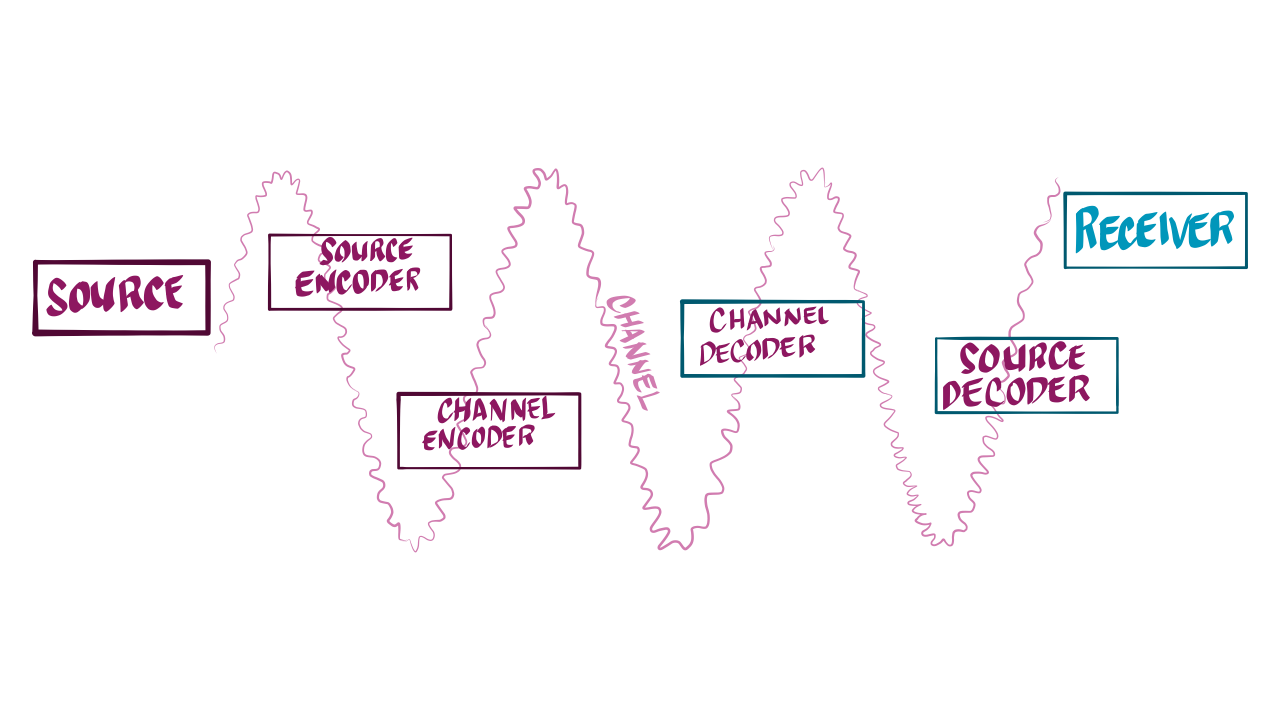
\includegraphics[width=0.9\textwidth]{Figures/Source_Destination.png}
\caption{Representation of the scheme of communication. In the image the noise in the channel is represented by the noise wavy connection between the parts in the communication. }
\label{CH2:Channel_communication}
\end{figure}
\\
Here we will consider codes in communication scenario, as the one showed in figure \ref{CH2:Channel_communication}, meaning that there will be a sender who wants to send $k$ message symbols over a noisy channel and there will be a receiver who has to correct possible errors over the sent code to fully interpret it. The sender will first encodes the $k$ message symbols into $n$ symbols. The receiver then tries to recover the original $k$ message symbols. thus, encoding is the process of adding redundancy and decoding is the process of removing errors and the communication can only be done over the channel\cite{mackay_information_2003}. The most fundamental question one can ask is what will be the relation between the amount of redundancy and the errors that can be corrected, and in order to answer this question we will provide some useful definitions.\\
\section{Some basic definitions}
\begin{definition}[Code]
A code of block $C$ length $n$ over an alphabet $\Sigma$ is a subset of $\Sigma^n$.  If $|\Sigma|=q$, we say that $C$ is a q-ary code.
\end{definition}
it is worth mention that, associated with a code there is also an encoding map $E$ which maps the message set $\mathcal{M}$, identified in some canonical way with $\{1,2,\ldots,|C|\}$ say, to code words belonging to $\Sigma^N$, and thus we have to understand the code as the image of the encoding map\cite{jaynes_probability_2003}.
\begin{definition}[Dimension of a code]
Given a code $C\subset\Sigma^n$, its dimension is given by
  \begin{equation}
  k \stackrel{\mathrm{def}}{=} \log _{q}|C|,
  \label{CH2:diemnsion_of_code}
  \end{equation}
 \end{definition}
An interesting fact about defining  the dimension of the code in this way is that implicitly it is telling us that when working with codes exponential growth will be always taken into account.\\
We have to provide here a way to measure the amount of redundancy in a given message.
	\begin{definition}[Rate of a code]
	The rate of a code with dimension $k$ and block length $n$ is given by 
	\begin{equation}
		R \stackrel{\text { def }}{=} \frac{k}{n},
		\label{CH2:Rate_of_code}
	\end{equation}
	\end{definition}
this definition is nothing but the average amount of non redundant information each of the $n$ symbols transmitted over the channel.\\ However, an alternative, and more general way of defining this is via the size of the code and the alphabet as
\begin{equation}
R(C)=\frac{\log |C|}{n \log |\Sigma|}.
\end{equation}

\begin{definition}[Hamming distance]
  The Hamming distance between two strings $x$ and $y$ of the same length over a finite alphabet $\Sigma$, denoted $\Delta(x,y)$, is defined as the number of positions at which the two strings differ, i.e, $\Delta(x,y) = |\{i| x_i \neq y_i\}|$. The fractional Hamming distance or relative distance between $x,y\in \Sigma^n$ is given by $\delta(x,y) = \frac{\Delta(x,y)}{n}$.
 \end{definition}
It is trivial to check that the Hamming distance defines a metric on $\Sigma^n$.
\begin{definition}
\textbf{Hamming weight:} The Hamming weight of a string $x$ over alphabet $\Sigma$ is defined as the number of non-zero symbols in the string. More formally, the Hamming weight of a string $\mathcal{W}(x) = |\{i| x_i \neq 0\}|$. Note that $\mathcal{W}(x-y) = \Delta(x,y)$.
\end{definition}
Given a string $x\in\Sigma^{N}$, the Hamming ball of radius $r$ around $x$ is the set $\{y\in\Delta^n | \Delta(x,y)\leq r\}$.\\
The minimum distance, or simply distance, of a code $C$, denoted $\Delta(C)$, is defined to be the minimum Hamming distance between two distinct code words of $C$. That is
\begin{definition}[Minimum distance]
 The minimum distance, or simply distance, of a code $C$, denoted $\Delta(C)$, is defined to be the minimum Hamming distance between two distinct code words of $C$. That is
\begin{equation}
\Delta(C)=\min _{c_{1}, c_{2} \in C \atop c_{1} \neq c_{2}} \Delta\left(c_{1}, c_{2}\right).
\end{equation}
In particular, for every pair of distinct code words in $C$ the Hamming Distance between them is at least $\Delta(C)$
\end{definition}

The relative distance of $C$, denoted $\delta(C)$, is the quantity $\frac{\Delta(C)}{N}$, where $N$ is the block length of $C$. Thus any two code words of $C$ differ in at least a fraction $\Delta(C)$.
\begin{definition}[Notation]
 A q-ary code of block length $N$ and dimension $k$ will be referred to as an $[N,k]_q$ code. Further, if the code has minimum distance $d$, it will be referred to as an $[N,k,d]_q$ code. When the alphabet size $q$ is clear from the context, or not very relevant to the discussion, we omit the subscript.
\end{definition}

Up to this point we have only described specific codes, codes with fixed block length and dimension. However, since we are interested in the asymptotic behaviour, it turns out to be more useful the study of families of codes instead of an specific code.

\begin{definition}[Family of Codes]
 Let $q\geq 2$. let $\{n_i\}_{i\geq 1}$ be and increasing sequence of block lengths and suppose there exists sequences $\{k_i\}_{i\geq 1}$ and $\{d_i\}_{i\geq 1}$ such that for all $i\geq 1$ there exist an $[n_i,k_i,d_i]_q$ code $C_i$. then the sequence $C=\{C_i\}_{i\geq1}$ is a family of codes. The rate of C is defined as
\begin{equation}
R(C)=\lim _{i \rightarrow \infty}\left\{\frac{k_{i}}{n_{i}}\right\},
\label{CH2:Rate_of_family_code}
\end{equation}
and the relative distance of $C$ is defined as
\begin{equation}
\delta(C)=\lim _{i \rightarrow \infty}\left\{\frac{d_{i}}{n_{i}}\right\},
\label{CH2:Relative_distance_of_family_code}
\end{equation}
from now on whenever we talk about a code we are implicitly referring to a family of codes.\\
\end{definition}
For the purpose of this work, we are going to focus on a particular class of codes, name minimum distance code. This special kind of codes came to our interest since they seem to appear naturally when study typical Fermionic states. We will then show some of the main results on this particular kind of codes to after show how this results could be extended to our particular case.\\
When we talk about codes of minimum distance $d$ we refer to codes which have the property that for every pair $x,y$ of codewords we have that
\begin{equation}
\Delta(x,y) =d,
\end{equation}


and therefore, the its relative distance $\delta$ is given by $N\delta=d$.\\
when working with this kind of codes one may wonder what is the best rate we can achieve. Particularly we are going to show 3 results, 1 positive and 2 negative results\footnote{Note that a negative result refer to an upper bound on the rate, meaning that the maximum achievable rate we could get can not exceed some value. Whereas a positive result refer to  lower bound on the rates we can achieve.}. Even though there are other known bounds, we will not talk about others but Gilbert-Varshamov, Hamming and Plotkin bounds, the reason for this is due to the fact that the other bound apply for large enough alphabets, so for binary codes we are not interested at all in these kind of bounds\cite{mackay_information_2003}.\\
\begin{figure}
\centering
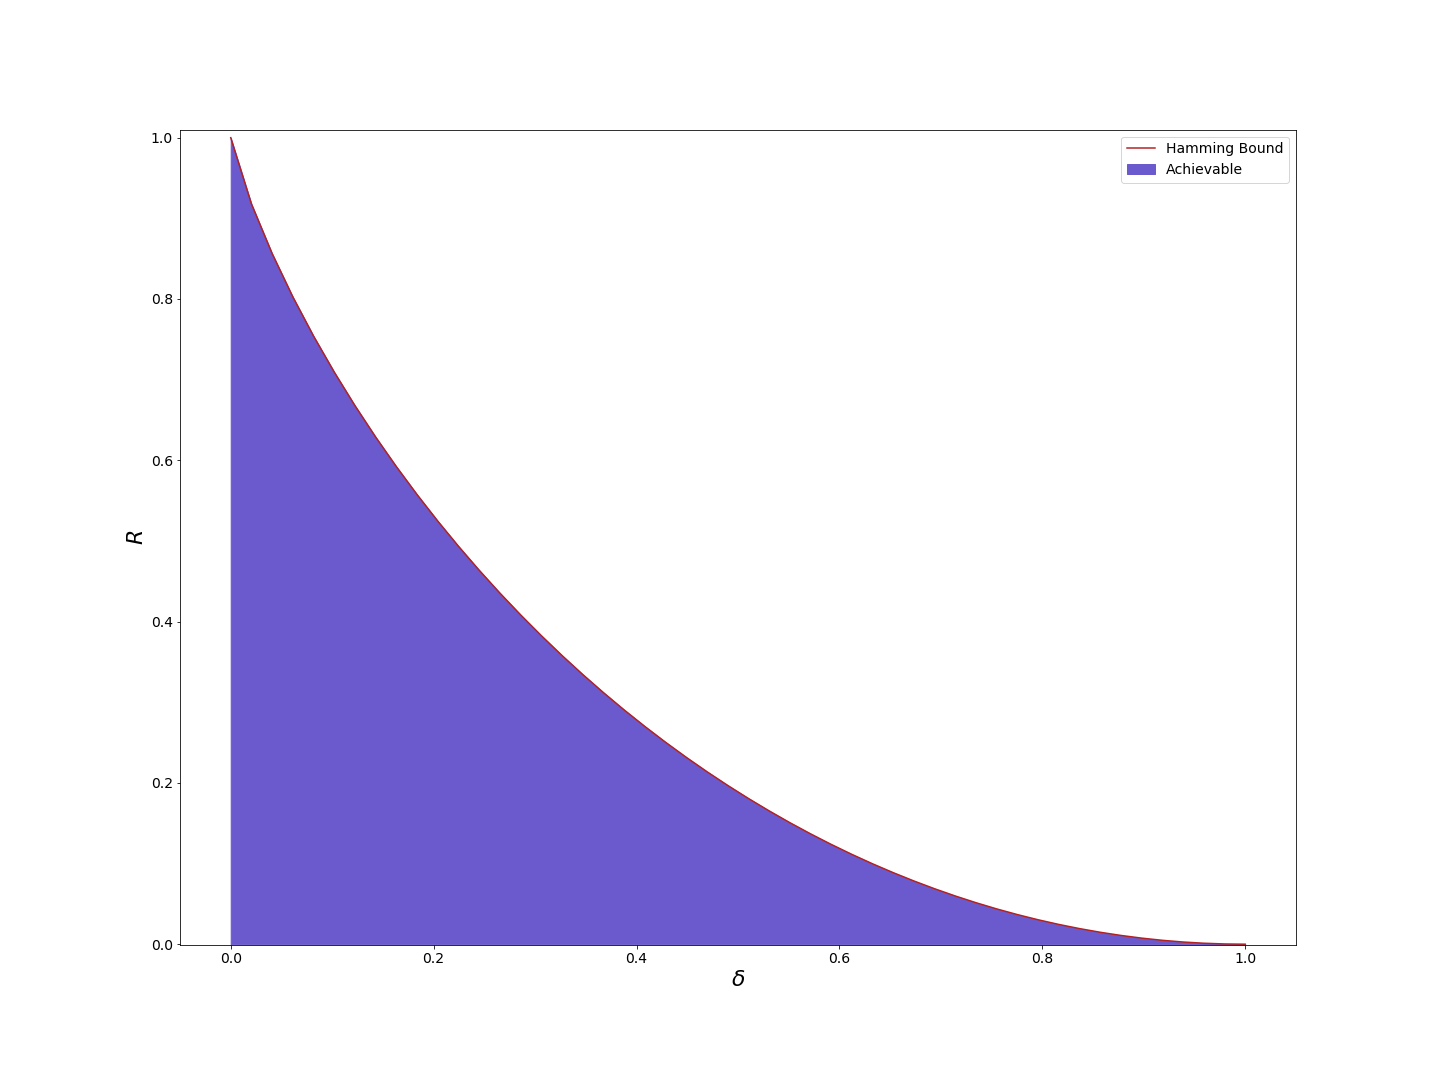
\includegraphics[width=0.7\textwidth]{Figures/Hamming_bound.png}
\caption{An illustration of the Hamming bound for the case of $q=2$. Note any code above this bound could exist. The shaded region shows the codes that could exist.  }
\end{figure}
\subsection{Hamming Bound (Sphere packing bound)}
\begin{definition}[Volume of Hamming ball]
Let $ q\geq2$ and $n \geq r \geq 1$ be integers. Then the volume of a Hamming ball of radius $r$ is given by
\begin{equation}
\operatorname{Vol}_{q}(r, n)=\left|B_{q}(\mathbf{0}, r)\right|=\sum_{i=0}^{r}\left(\begin{array}{l}
n \\
i
\end{array}\right)(q-1)^{i},
\label{CH2:Hamming_ball}
\end{equation}
where the choice of $\mathbf{0}$ as the center of the Hamming ball is chosen arbitrary, since the volume of the Hamming ball is independent of its center.
\end{definition}
It is simple to show that
\begin{equation}
\frac{k}{n} \leq 1-\frac{\log _{q} \operatorname{Vol}_{q}\left(\left\lfloor\frac{d-1}{2}\right\rfloor, n\right)}{n},
\label{CH2:Hamming_bound_1}
\end{equation}
where the volume in \eqref{CH2:Hamming_bound_1} correspond to the definition in\eqref{CH2:Hamming_ball}. With some algebra and using the Stirling asymptotic approximation one can show that
\begin{equation}
\operatorname{Vol}_{q}\left(\left\lfloor\frac{d-1}{2}\right\rfloor, n\right) \geq q^{H_{q}\left(\frac{\delta}{2}\right) n-o(n)},
\end{equation}
where the latter inequality immediately provide us an upper bound on the rate
\begin{equation}
R \leq 1-H_{q}\left(\frac{\delta}{2}\right)+o(1).
\label{CH2:Hamming_bound_2}
\end{equation}

The inequality in \eqref{CH2:Hamming_bound_2} is known as the Hamming Bound.

\subsection{Plotkin Bound}
\begin{definition}[Plotkin Bound]
The following holds for any code $\mathcal{C}\subset [q]^n$ 
\begin{itemize}
\item If $d=\left(1-\frac{1}{q}\right) n,|\mathcal{C}| \leq 2 q n$.
\item If $d>\left(1-\frac{1}{q}\right) n,|\mathcal{C}| \leq \frac{q d}{q d-(q-1) n}$.
\end{itemize}
Note that the Plotkin Bound implies that a code with relative distance $\delta\geq 1-1/q$, must necessarily have $R=0$.
\end{definition}

\begin{definition}
For any q-ary code with relative distance $0 \leq \delta \leq 1-\frac{1}{q}$,
\begin{equation}
R \leq 1-\left(\frac{q}{q-1}\right) \delta+o(1).
\label{CH2:Plotkin_bound}
\end{equation}
\end{definition}

\begin{figure}
\centering
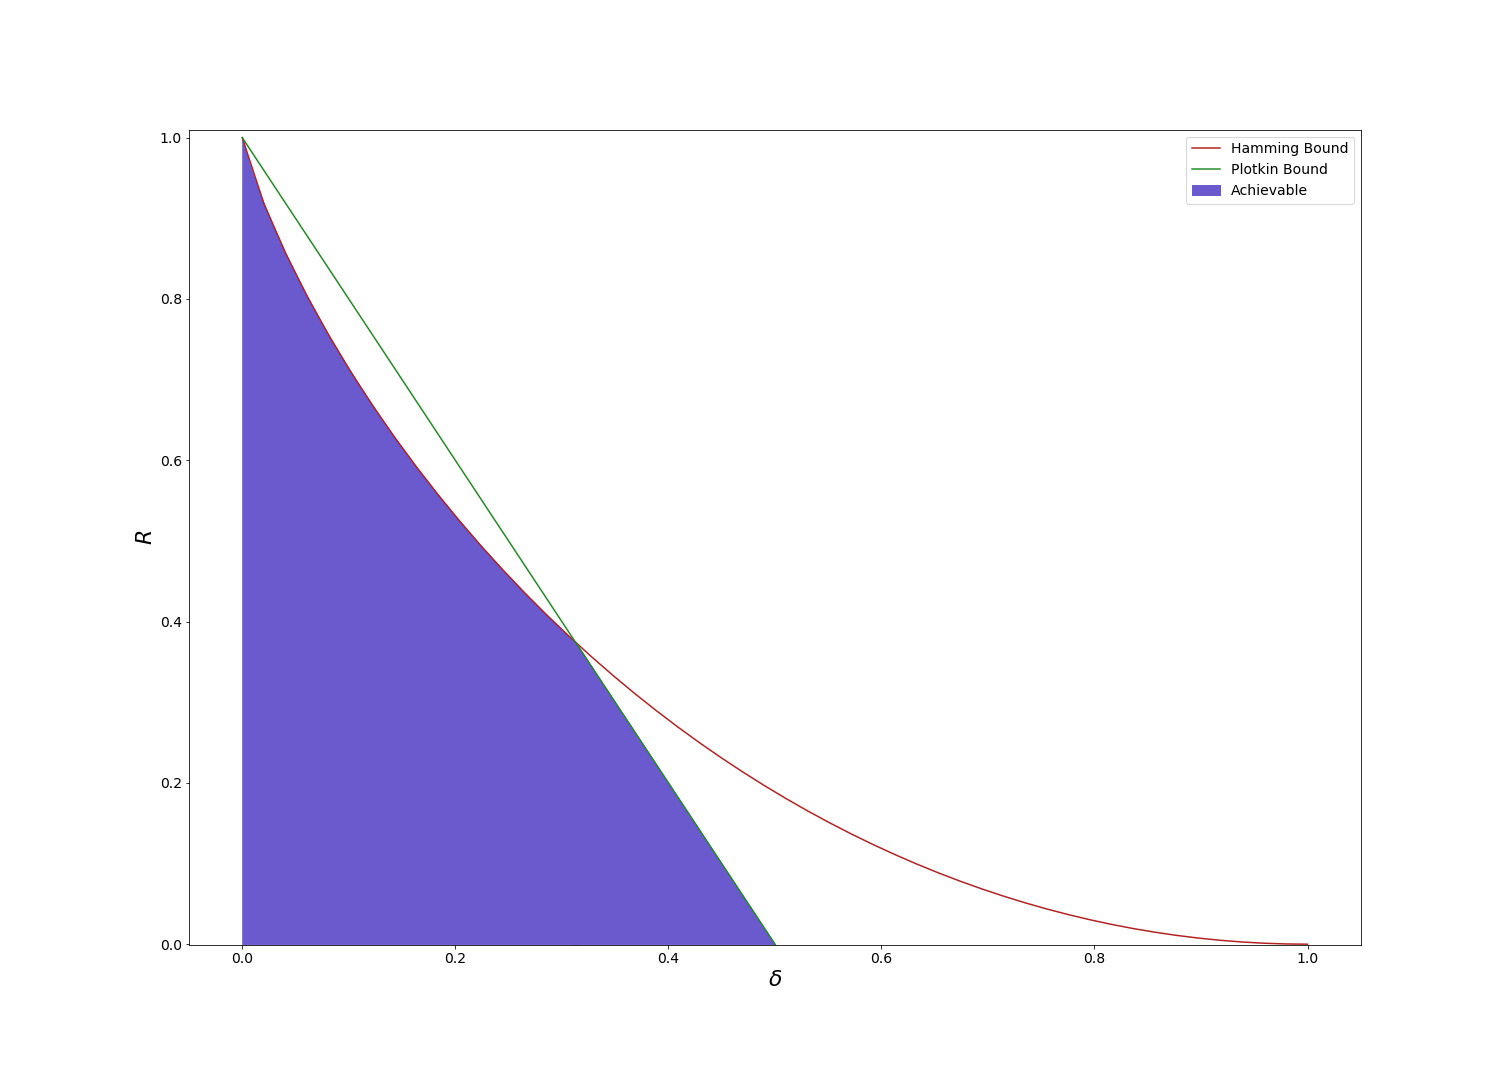
\includegraphics[width=0.7\textwidth]{Figures/Hamming_plotkin_bound.png}
\caption{An illustration of Plotkin and Hamming bounds for the case of $q=2$.  For this case the shaded region changes indicating us that there are not codes with $R>0$ when $\delta=1-1/q$ .}
\end{figure}

To illustrate the proof of this bound we can consider the distance $d=n\delta$. So we can shorten the codewords and group them in a way such that they agree on the first $n-n'$ symbols, with $n^{\prime}=\left\lfloor\frac{q d}{q-1}\right\rfloor-1$. Then in particular for any $x\in [q]^{n-n'}$, define the prefix code
\begin{equation}
\mathcal{C}_{\mathbf{x}}=\left\{\left(c_{n-n^{\prime}+1}, \ldots c_{n}\right) \mid\left(c_{1} \ldots c_{N}\right) \in \mathcal{C},\left(c_{1} \ldots c_{n-n^{\prime}}\right)=\mathbf{x}\right\}.
\end{equation}
for all $x,\ \mathcal{C}_{x}$, has distance $d$ as $\mathcal{C}$ has distance $d$. Additionally, it has block length $n^{\prime}<\left(\frac{q}{q-1}\right) d$, and thus $d>\left(1-\frac{1}{q}\right) n^{\prime}$. From the Plotkin bound, this implies that
\begin{equation}
\left|\mathcal{C}_{\mathbf{x}}\right| \leq \frac{q d}{q d-(q-1) n^{\prime}} \leq q d,
\end{equation}
where the second inequality follows from the fact that $q d-(q-1) n^{\prime}$ is an integer.\\
Note that from the definition of $\mathcal{C}_{x}$
\begin{equation}
|\mathcal{C}|=\sum_{\mathbf{x} \in[q]^{n-n^{\prime}}}\left|\mathcal{C}_{\mathbf{x}}\right|,
\end{equation}
which tell us that 

\begin{equation}
\left.|\mathcal{C}| \leq \sum_{\mathbf{x} \in[q]^{n-n^{\prime}}} q d=q^{n-n^{\prime}} \cdot q d \leq q^{n-\frac{q}{q-1} d+o(n)}=q^{n\left(1-\delta \cdot \frac{q}{q-1}+o(1)\right)}\right.,
\end{equation}

in other words this provides another upper bound to the rate given by
\begin{equation}
R \leq 1-\left(\frac{q}{q-1}\right) \delta+o(1)
\label{CH2:Plotkin:bound_rate}
\end{equation}
To close this part we will show the latter but positive result which provide us  lower bound on the code rates, Gilbert Varshamov bound.
\subsection{Gilbert Varshamov Bound}
We now switch gears to provide a positive result. We will only provide the main ideas for the proof of this result an we will discuss why this result turn out to be one of the most important results.
\begin{definition}[Gilbert-Varshamov Bound]
Let $q\geq 2$. For every $0 \leq \delta<1-\frac{1}{q}$ and $0<\varepsilon \leq 1-H_{q}(\delta)$. There exist a code with rate $R \geq 1-H_{q}(\delta)-\varepsilon$ and relative distance $\delta$.
\label{CH2:Definition_Gilbert_Varshamov}
\end{definition}

\begin{figure}
\centering
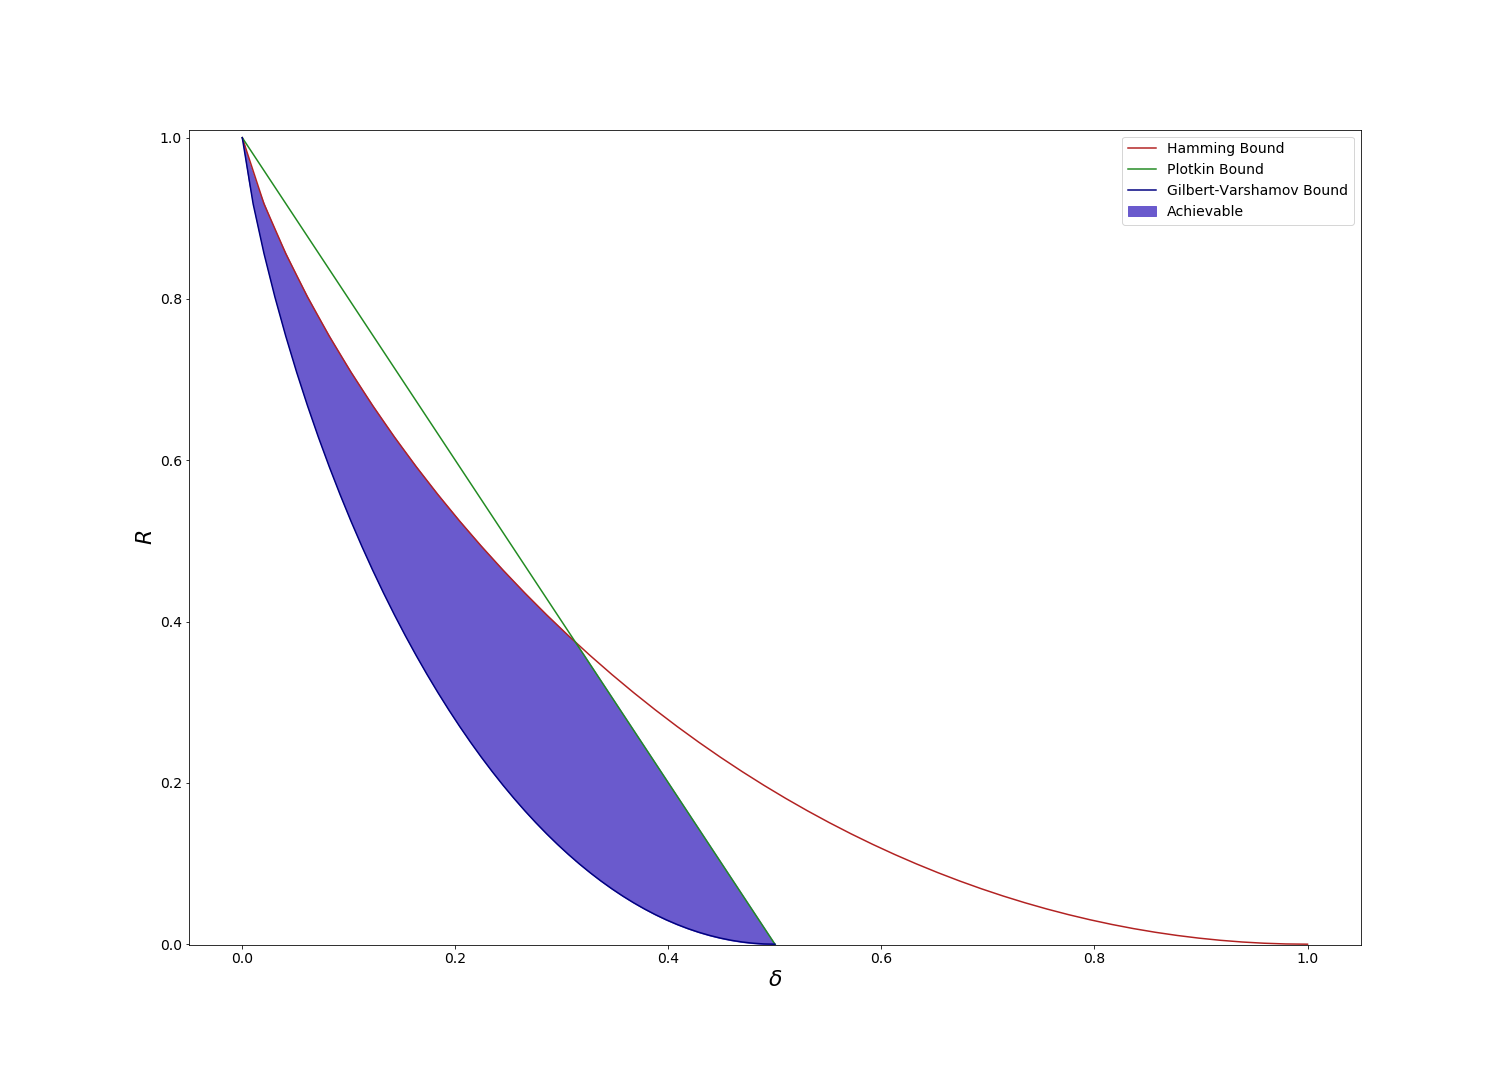
\includegraphics[width=0.7\textwidth]{Figures/Hamming_plotkin_Gilbert_bound.png}
\caption{An illustration of 3 bounds Hamming, Plotkin and Gilbert-Varshamov for the case of $q=2$. The lower bound correspond to the Gilvert-Varshamov Bound whereas the other 2 are the upper bound for the rate.}
\end{figure}

To provide a main idea about the proof we can consider a greedy approach. First we start with an empty code $\mathcal{C}$ and we keep adding vectors that are not in $\mathcal{C}$ and that have Hamming distance at least $d$ from all the existing codewords in $\mathcal{C}$. Notice that by doing so we can assure that we will never add a vector $c$ that will make that will make the distance of $\mathcal{C}$ fall below $d$. Indeed it is easy to see that after doing so, we have
\begin{equation}
\bigcup_{\mathbf{c} \in C} B(\mathbf{c}, d-1)=[q]^{n},
\label{CH2:Gilbert_Varshamov_1}
\end{equation}
this is easily checked, because if it was not true, then there would exist a vector $\mathbf{v} \in[q]^{n} \backslash C$, such that $\Delta(\mathbf{v}, \mathbf{c}) \geq d$ and therefore $\mathbf{v}$ can be added. How ever, this would contradict the fact that we have finished the procedure. So

\begin{equation}
\bigcup_{c \in C} B(\mathbf{c}, d-1) \mid=q^{n}.
\label{CH2:Gilbert_Varshamov_2}
\end{equation}
It isn't hard to see that
\begin{equation}
\sum_{\mathbf{c} \in C}|B(\mathbf{c}, d-1)| \geq\left|\bigcup_{\mathbf{c} \in C} B(\mathbf{c}, d-1)\right|,
\label{CH2:Gilbert_Varshamov_3}
\end{equation}

which implies that
\begin{equation}
\sum_{\mathbf{c} \in C}|B(\mathbf{c}, d-1)| \geq q^{n},
\label{CH2:Gilbert_Varshamov_4}
\end{equation}
but as mentioned before, the volume of the Hamming ball is translation invariant,

\begin{equation}
\sum_{\mathbf{c} \in C} \operatorname{Vol}_{q}(d-1, n) \geq q^{n}.
\label{CH2:Gilbert_Varshamov_5}
\end{equation}

Since $\sum_{\mathbf{c} \in C} V o l_{q}(d-1, n)=V o l_{q}(d-1, n) \cdot|C|$ 

\begin{equation}
\begin{aligned}
|C| & \geq \frac{q^{n}}{\operatorname{Vol}_{q}(d-1, n)} \\
& \geq \frac{q^{n}}{q^{n H_{q}(\delta)}} \\
&=q^{n\left(1-H_{q}(\delta)\right)}.
\end{aligned}
\label{CH2:Gilbert_Varshamov_final}
\end{equation}

And therefore concluding the proof. It is worth mention that this way of proceeding the code have not any special structure but as one might think this algorithm will take exponentially long time to finish. How ever, one may wonder if there is a special kind of code that also achieve this rate. Indeed is possible to show that random linear codes lies, with high probability, on the Gilbert-Varshamov Bound. To pick a linear random code we only need pick a random $k\times n $ matrix, in which each entry is chosen uniformly and independently at random according to its alphabet\cite{mackay_information_2003,jaynes_probability_2003}. Aside from these result providing some bounds on the rate of the minimum distance codes. We are interested in the performance of a special kind of random codes, more specifically binary codes over a binary-symmetric channel (BSC). In here we derive the minimum distance, distance distribution and error exponent of a typical random code (TRC) from a random code ensemble (RCE), as well as the one correspondent to a typical linear code (TLC) from a linear code ensemble (LCE) \cite{barg_random_2002}. As mentioned by \textit{A Barg, and G. D. Forney, Jr} most of the important of these results are expressed in terms of the Gilbert-Varshamov distance  $\delta_{GV}(R)$.
\subsection{Error Exponents for Random Minimum Distance Codes}
It is very well known that on a BSC with crossover probability $p$, the channel capacity is $C=1-H_2(p)$ \footnote{We will be using the notation $\mathcal{H}$ to refer to the binary entropy $\mathcal{H}\equiv H_2$ }. The error coding exponent $E_r(R)$ is positive for $0\leq R < C$ and given by \cite{gallager_low-density_1962,gallager_information_1968}.
\begin{equation}
E_{r}(R)=\left\{\begin{array}{ll}
R_{0}-R, & 0 \leq R \leq R_{\text {crit }} \\
E_{\mathrm{sp}}(R), & R_{\text {crit }} \leq R \leq C
\end{array}\right.,
\end{equation}
where $R_0$,  $R_{\text {crit }}$ and $E_{\mathrm{sp}}(R)$, are known as cutoff rate, critical rate and the sphere-packing exponent respectively. In \cite{gallager_random_2006} Gallager has shown that the random coding exponent is the true error exponent for the RCE   on any discrete memoryless channel. Here we will show the main results provided in \cite{barg_random_2002} and we will provide the ideas to derive these results, as we will show later this ideas of error exponents will be quite helpful to understand how it is possible to make a connection between minimum distance codes and typical Fermionic  states.
\subsubsection{Random Binary Codes}
Consider a binary code $C$ of length $N$ and rate $R$ bits per symbol is a set of $M=2^{NR}$. For the case of RCE one compute the probability that by taking a random codeword $\mathbf{x}_i$ of length $N$ it would have Hamming distance $d=N\delta$ from an arbitrary binary $N-$tuple $\mathbf{b}$ and see that it will be independent of $\mathbf{b}$ and equals to
\begin{equation}
\text{Pr}\{d_H(\mathbf{x}_i,\mathbf{b})=d\}={N\choose d} \tilde{p}^d (1-\tilde{p})^{N-d},
\end{equation}
where $\tilde{p}$ corresponds to the probability of having a one. Under this RCE, two distances $d_H(\mathbf{x}_i,\mathbf{x}_j)$ and $d_H(\mathbf{x}_{i'},\mathbf{x}_{j'})$ are independent random variables. So if we consider the number of unordered pairs of codewords $(\mathbf{x}_i,\mathbf{x}_j)$ with $i\neq j$ in $C$ at a distance $d$ apart
\begin{equation}
S_{\mathcal{C}}(d)=\sum_{i=0}^{M-1} \sum_{j=0}^{i-1} \Phi\left\{d_{H}\left(\boldsymbol{x}_{i}, \boldsymbol{x}_{j}\right)=d\right\},
\end{equation}
where $\Phi\left\{d_{H}\left(\boldsymbol{x}_{i}, \boldsymbol{x}_{j}\right)=d\right\}$ is equal to 1 if the condition $d_H(\mathbf{x}_i,\mathbf{x}_j)$ is satisfied and $0$ otherwise. For the case of RCE on a BSC $S_{\mathcal{C}}(d)$ is a sum of ${M\choose 2}$ pairwise independent, identically distributed random variables, so we have

\begin{equation}
\mathrm{E} S_{\mathcal{C}}(d)=\left(\begin{array}{c}
M \\
2
\end{array}\right) \mathrm{E} \Phi \doteq 2^{N(2 R-1+\mathcal{H}(\delta))}.
\end{equation}
Therefore we are ready to state the following theorem
\begin{theorem}[Minimum distance in RCE]
For $0\leq R< 1/2$ and any $\varepsilon>0$, the probability that a code length $N$ and rate $R$ from the RCE has relative minimum distance less than $\delta_{GV}(2R)-\varepsilon$ goes to zero exponentially as $N\to \infty$. For $0\leq R < 1$, if $d=N\delta$ is such that
\begin{equation}
\delta_{GV}(2R)+\varepsilon \leq \delta \leq 1- \delta{GV}(2R) - \varepsilon,
\end{equation}
then the probability that the number of codeword pairs at a distance d satisfies $S_{\mathcal{C}}(d) \doteq 2^{N(2 R-1+\mathcal{H}(\delta))}$ goes to one as $N\to \infty$.
\end{theorem}

\begin{proof}
For a given value of the code value of the code rate $R$ we can choose $d$ such that $d/N\to\delta \leq \delta_{\mathrm{GV}}(2 R)-\varepsilon$. Then
\begin{equation}
\operatorname{Pr}\left\{S_{\mathcal{C}}(d) \geq 1\right\} \leq \mathrm{E} S_{\mathcal{C}}(d) \doteq 2^{-N(1-\mathcal{H}(\delta)-2 R)} \rightarrow 0,
\end{equation}
which in other words it tell us that with probability differing from $1$ by an exponentially falling quantity, there will be no pairs at distance $d$. Notwithstanding this result, if $\delta_{\mathrm{GV}}(2 R)+\varepsilon<\delta<1-\delta_{\mathrm{GV}}(2 R)-\varepsilon$, then $1-\mathcal{H}(\delta)<2R$ and the average of number of pairs $\mathrm{E} S_{\mathcal{C}}(d)$ at a distance $d$ is exponentially large. To see this, we can use the Chebyshev inequality, so for any $\delta>0$, we have 
\begin{equation}
\operatorname{Pr}\left\{\left|S_{\mathcal{C}}(d)-\mathrm{E} S_{\mathcal{C}}(d)\right| \geq\left(\begin{array}{c}
M \\
2
\end{array}\right) \alpha\right\} \leq \frac{\mathrm{E} \Phi}{\left(\begin{array}{c}
M \\
2
\end{array}\right) \alpha^{2}},
\end{equation}
by choosing $\alpha \doteq 2^{-N(1-\mathcal{H}(\delta)+\Delta)}<\mathrm{E} \Phi$ for any $\Delta>0$, we have
\begin{equation}
\operatorname{Pr}\left\{\left|S_{\mathcal{C}}(d)-\mathrm{E} S_{\mathcal{C}}(d)\right|>\left(\begin{array}{c}
M \\
2
\end{array}\right) \alpha\right\}\leq \frac{2 \mathrm{E} \Phi}{M(M-1) \alpha^{2}} \doteq 2^{-N(2 R-1+\mathcal{H}(\delta)-2 \Delta)}.
\end{equation}
The exponent on the right-hand side can be made positive by choosing $\Delta$ small enough. This establishes the fact that $S_{\mathcal{C}}(d)\doteq 2^{N(2 R-1+\mathcal{H}(\delta))}$ for the chosen value of $d$ with probability tending to one as $N\to\infty$.
\end{proof}
\subsubsection{Random Linear Codes}
A binary linear code $C$ of length $N$ and rate $K/N$ is a set of $M=2^K$ binary $N$-tuples that is generated by $K$ $N-$tuples $\mathbf{g}_j$, $1\leq k \leq K$. This is
\begin{equation}
\mathbf{x}(u)=\Sigma_k \mathbf{u}_k \mathbf{g}_j,
\end{equation}
where $\mathbf{u}$ is an arbitrary binary $K-$tuple. Here we will be considering the case in which each of the $2^{NK}$ matrices are chosen with equal probability. For the case of linear codes, the distribution of distance $\{d_H(\mathbf{x}_i,\mathbf{x}_j),i\neq j\}$ from any given codeword $\mathbf{x}_i$ is independent of $i$. The average distance distribution of a linear code $C$ therefore reduces to
\begin{equation}
\mathcal{N}_{\mathcal{C}}(d)=\sum_{j \neq i} \Phi\left\{d_{H}\left(\boldsymbol{x}_{i}, \boldsymbol{x}_{j}\right)=d\right\} \quad(d=1,2, \ldots, N),
\label{CH2:RLC_number of codewords}
\end{equation}
where $\mathbf{x}_i$ is an arbitrary codeword. Typically, $\mathbf{x}_i$ is taken as the all zero codeword $\mathbf{0}=\mathbf{x(0)}$. If $(\mathbf{u}_j,\mathbf{u}_k)$ is any pair distinct non-zero $K-$tuples, then the corresponding codewords $(\mathbf{x}(\mathbf{u}_j),\mathbf{x}(\mathbf{u}_k))$ are a pair of independent random binary $N-$tuples. It follows that two distinct distances $d_H(\mathbf{x}_i,\mathbf{x}_j)$ and $d_H(\mathbf{x}_i,\mathbf{x}_k)$ from a given codeword $\mathbf{x}_i$ are pairwise-independent and distributed as in the RCE. In particular 
\begin{equation}
\operatorname{Pr}\left\{d_{H}\left(\boldsymbol{x}_{i}, \boldsymbol{x}_{j}\right)=N \delta\right\} \doteq 2^{-N(1-\mathcal{H}(\delta))},
\end{equation}
for any $d=N\delta$, the quantity $\mathcal{N}_{\mathcal{C}}(d)$ in \eqref{CH2:RLC_number of codewords} is a sum of $M-1\doteq 2^{NR}$ pairwise-independent, identically distributed random variables with mean $E\Phi\doteq 2^{-N(1-mathcal{H}(\delta))}$. Its mean value is therefore equal to

\begin{equation}
\mathcal{N}_{\mathrm{LCE}}(d) \doteq 2^{N(R-1+\mathcal{H}(\delta))}.
\end{equation}
Therefore we say that the relative minimum distance of a code chosen at random from the LCE will be, with probability $1-2^{-\Omega(N)}$, approximately equal to the $GV$ relative distance $\delta_{GV}(R)$.\\
In summary, the typical minimum distance in the LCE is better than that in the RCE because the minimum of only $M-1$ pairwise-independent distances, whereas in the RCE it is the minimum of ${M\choose 2}$ pairwise independent distances.\\
Up to this point one may be wonder how all this theory of correcting errors and minimum distance codes are connected to our problem. In following section we are going to show how this connection emerge as a natural consequence of the structure in the Clifford algebra and therefore provide an explanation of what we named as ``Super-Orthogonality''.
\section{Mechanism behind typicality as a correction error method.}
As we mentioned in the first chapter, we are interested in study the behaviour of states which are close in energy. First we will show why it is possible to study ``Ultra Orthogonality'' for Fermionic states in two possibilities. The first one is in terms of minimum distance codes and we will see that ``Ultra Orthogonality'' turns out to be an exact result. For the second part, we deduce its correspondent exponent error. For the last part, we will tackle the problem when we can not work over a minimum distance and we will show how ``Ultra orthogonality'' can be acting over this specific case. Even though for this case we were not able to generalised this to every Fermionic system, we will discuss why this result should holds in general.\\
\subsection{``Ultra Orthogonality'' on Fermions}
To start this part we want to recapitulate a couple of things. First, as we showed in equation \eqref{CH1:expansion_5}, when we take the partial trace the remaining cross terms  will be of our interest. When we discuss the property of Ultra Orthogonality, we stated that the cross terms of $\operatorname{Tr}_{E}\ket{E_n}\bra{E_m}$ should be the ones that had to be near to zero, in order for thermalisation to occur on the specific case we discussed in chapter $1$. Here we are going to formalise all these ideas.\\
We can start by choosing an arbitrary state such that it can be decomposed in its vectors of the Fock basis as\footnote{Note that we can use the Fock basis since it is naturally the basis in which we diagonalise our Hamiltonian, therefore it is an energy basis as well.}
\begin{equation}
\ket{\psi} = \sum_{\vec{n}}\psi(\vec{n})\ket{\vec{n}}.
\end{equation}
Therefore we are interested in studying the terms of the form\footnote{Here we denote the partial trace by $\operatorname{Tr}_{N/L}$ meaning that for the corresponding sequence of length $N$ in the Fock Space we take the respective $L$ elements, meaning that $N-L$ elements will be regarded as our environment.}
\begin{equation}
\hat{X}_{ij} \doteq \operatorname{Tr}_{E}\left(\ket{\vec{n}_i}\bra{\vec{n}_j}\right) \equiv \operatorname{Tr}_{N/L}\left(\ket{\vec{n}_i}\bra{\vec{n}_j}\right).
\end{equation}
What Ultra orthogonality tell us is that this term has to zero or in the worst scenario something of the order of 
fluctuations. Since we are working on the very special case of Quadratic Hamiltonian describing Fermionic systems, we recall the fact that the operators are generated by the Majorana operators, and form the so called Clifford algebra, described in section 2.2. We also saw that these operators can be mapped to the Grassman variables, which allow us to compute things like observables. Taking into account that we started with an space in which we had to deal with $N$ Pauli operator and we changed to a new space in which we work with $2N$ spinless operators and the fact that the most general  function we can built over the Grassman algebra is polynomial of the Grassmann variables. Thus we construct a function of the Grassman variables which takes two binary sequences ($\vec{x},\vec{y}$), $x_i,y_i \in \{0,1\}$, lets call it $\gamma(\vec{x},\vec{y})$. the reason for defining this function is that we are going to describe the system in the space of size $L$ with its correspondent operators, meaning that these sequences can not be arbitrary, they must have to be sequences such that after its first $L$ elements, they must have only zeros. To illustrate this consider the following example, let $\vec{x}=(0100\ldots 0)$, $\vec{y}=(1100\ldots 0)$, here $L=3$, so our function will be described by\footnote{Here we have changed the original notation given in \eqref{CH2:majorana} and change it by 
\begin{equation}
\hat{c}_{2j-1}\rightarrow \gamma_{j} , \qquad \hat{c}_{2j}\rightarrow \gamma_{N+j},
\end{equation}
for the case of $N$ operators.
}
\begin{equation}
\gamma(\vec{x},\vec{y}) = \gamma_1^{x_1=0} \gamma_{4}^{y_1=1} \gamma_{2}^{x_2=1} \gamma_{5}^{y_2=1} \gamma_{3}^{x_3=0} \gamma_{6}^{y_3=1} = \gamma_{4}\gamma_{2}\gamma_{5}\gamma_{6},
\end{equation}
Note that in this way we are able to write any product of Grassmann operators. in general, for two sequences, and a fixed size $L$ this function will be given by
\begin{equation}
\gamma(\vec{x},\vec{y}) = \gamma_1^{x_1} \gamma_{L+1}^{y_1} \gamma_{2}^{x_2} \gamma_{L+2}^{y_2}\ldots \gamma_{L}^{x_L} \gamma_{2L}^{y_L},
\end{equation} 
where this function has the property that
\begin{equation}
\gamma(\vec{x},\vec{y})\gamma(\vec{x}',\vec{y}') = e^{i\phi(\vec{x},\vec{y},\vec{x}',\vec{y}')} \gamma(\vec{x}+\vec{x}',\vec{y}+\vec{y}').
\label{CH2:my_relation_delta}
\end{equation}
 The phase appear as a consequence of the anti-commutation relation and $\phi(\vec{x},\vec{y},\vec{x}',\vec{y}')$ is a function that would depend on the weight of the sequences $\vec{x},\vec{y},\vec{x}'$and $\vec{y}'$.\\
This provide a set of operators that live in the space of size $L$, and that will allow us to expand our operator $\hat{X}_{ij}$,\footnote{For illustrate these ideas we first suppose we have the operators in order. However, we will generalise it later.}
\begin{equation}
\hat{X}_{ij} = \sum_{\vec{x},\vec{y}} f(\vec{x},\vec{y})\gamma(\vec{x},\vec{y}).
\end{equation}
Our task will then be to find the coefficient $f(\vec{x},\vec{y})$, this can be achieve by multiplying on both sides by $\gamma(\vec{x'},\vec{y'})$ and taking the trace over $L$
\begin{equation}
\operatorname{Tr}_L\left(\hat{X}_{ij}\gamma^{\dagger}(\vec{x}',\vec{y}')\right)=\sum_{\vec{x},\vec{y}}f(\vec{x},\vec{y}) \operatorname{Tr}_L\left(\gamma(\vec{x},\vec{y})\gamma^{\dagger}(\vec{x}',\vec{y}')\right).
\end{equation}
The right hand side of this equation can be combined with equation \eqref{CH2:my_relation_delta} and deduce that it will give us a delta ($\delta_{\vec{x}+\vec{x}'}\delta_{\vec{y}+\vec{y}'}$). Thus the coefficients $f(\vec{x},\vec{y})$ are given by
\begin{equation}
f(\vec{x}',\vec{y}') = \frac{1}{2^L}\operatorname{Tr_L}\left(\hat{X}_{ij}\gamma^{\dagger}(\vec{x}',\vec{y}')\right)=\frac{1}{2^L} \bra{\vec{n}_j}\gamma^{\dagger}(\vec{x}',\vec{y}')\ket{\vec{n}_i}.
\label{CH2:my_relation_coefficients}
\end{equation}
Thus we first have to know how the operators $\gamma$ acts over the states $\ket{\vec{n}_i}$, for this we recall the fact that the Hamiltonians are diagonalised via an orthogonal transformation which links what we call the spacial modes and the normal modes
\begin{equation}
\overbrace{\gamma_{i_1}\gamma_{i_2}\ldots\gamma_{i_k}}^{\text{Spacial modes}}= O_{i_1\alpha_1}O_{i_2\alpha_2}\ldots O_{i_k\alpha_k} \underbrace{\gamma_{\alpha_1}\gamma_{\alpha_2}\ldots\gamma_{\alpha_k}}_{\text{Normal modes}}.
\end{equation}
Note that this operators are diagonal over our $\vec{x}$'s and$\vec{y}$'s, which will allow us to operate over the states $\ket{\vec{n}_i}$.\footnote{By using the function $\gamma(\vec{x},\vec{y})$ there are two ways of getting an specific state $\ket{\vec{n}_i}$
\begin{equation}
\ket{n_i}=\gamma(\vec{n}_i,0)\ket{0}, \qquad \ket{n_i}=\gamma(0,\vec{n}_i)\ket{0}e^{i\phi(\vec{n_i})},
\end{equation}
therefore we can say that the $\vec{x}$'s takes the $0$ and turn them into a $1$, and the $\vec{y}$'s take $0$ and transform it into a one multiplied by a phase.
}. The equation \eqref{CH2:my_relation_coefficients} will be simplified to
\begin{equation}
\bra{\vec{n}_j}\gamma(\vec{x},\vec{y})\ket{\vec{n}_i}=\delta_{\vec{n}_i+\vec{x}+\vec{y},\vec{n}_j}e^{i\phi(\vec{n}_i,\vec{n}_j,\vec{x},\vec{y})},
\label{CH2:my_relation_coeficients_2}
\end{equation}
whereas the coefficients $f(\vec{x},\vec{y})$ will be given by
\begin{equation}
f(\vec{x},\vec{y}) = \frac{1}{2^L}\sum_{\vec{x}',\vec{y}'} \mathcal{U}_{\vec{x}\vec{x}'} \mathcal{V}_{\vec{y}\vec{y}'} \underbrace{\bra{\vec{n}_j}\gamma(\vec{x},\vec{y})\ket{\vec{n}_i}}_{\propto \delta_{\vec{n}_i+\vec{n}_j},\vec{x}+\vec{y}}.
\label{CH2:my_Relation_coeffitients_final}
\end{equation}
In equation \eqref{CH2:my_relation_coeficients_2} the term with the delta can be change by $\delta_{\vec{n}_i+\vec{n_j},\vec{x}+\vec{y}}$, an the reason to do so is because we are working with arithmetic mod $2$ and we can see that the term $\vec{n}_i+\vec{n}_j$ is nothing but the vector of differences, which means that the only values different than zero in this vector are when $n_{i_k}\neq n_{j_k}$. This result is extremely important because it tell us that when ever we work with states like $\hat{X}_{ij}$, if the vector of differences have more ones than the vector of differences $\vec{x}+\vec{y}$. Note that the vector of difference given by $\vec{x}+\vec{y}$ can have at most $L$ errors, which means that whenever the number of ones in the difference vector defined by the states $\vec{n}_i+\vec{n}_j$ exceeds $L$ the state $\hat{X}_{ij}$ will be immediately zero. This turns out to be an astonishing result and bring even more questions, like how likely is to have more than $L$ errors when $N\gg L$?, what happen when we have less errors is this quantity still small enough as we expected?. These questions will be tackled in a moment but something to stress is the fact that it is the branch point of our study. We will be first addressing the first question and afterwards we will talk about the second one.
\subsection{Codes of minimum distance constrained to an energy value}
Lets recapitulate a little more what we have done in the latter chapter. We define two binary sequences of excitations $\vec{n}_i$, $\vec{n}_j$, and the vector of differences $\vec{e}_{ij}=\vec{n}_i$+$\vec{n}_j$, we will denote the distance between these two binary sequences by
\begin{equation}
\begin{aligned}
d&=W(\vec{e}_{ij})\rightarrow \text{Weight of }\vec{e}_{ij} \\
&=d_{H}(\vec{n}_i, \vec{n}_j) \rightarrow \text{Hamming distance.}
\end{aligned}
\end{equation}
we show that there is a specific distance $d>L$ at which the state $\hat{X}_{ij}=\operatorname{Tr}_{N/L}\left(\bra{\vec{n}_i}\ket{\vec{n}_j}\right)$ is equal to zero $\hat{X}_{ij}$. This might sound quite familiar since it is connected to minimum distance codes and to see this more clearly consider a set of binary codewords
\begin{equation}
\mathcal{C}=\{\vec{x}^{(1)},\vec{x}^{(2)},\ldots,\vec{x}^{(2^k)}\} \quad \vec{x}\in\{0,1\}^{N},
\end{equation}
and size $|\mathcal{C}|=2^{NR}$, with $R=k/N$ as defined in \eqref{CH2:Rate_of_code}. Analogously, consider the Hilbert space
\begin{equation}
\mathcal{H}_{\mathcal{C}}=\operatorname{Span}\left(\ket{\vec{x}^{(1)}},\ket{\vec{x}^{(2)}},\ldots,\ket{\vec{x}^{(2^k)}}\right).
\end{equation}
It is easy to check that $|\mathcal{H}_{\mathcal{C}}|=|\mathcal{C}|=2^{NR}$. From the results showed from section $2.6$ we can assure that there exist a Hilbert space with dimension $\operatorname{dim}|\mathcal{H}_{\mathcal{C}}|=2^{N(1-\mathcal{H}(\ell))}$, where $\ell = L/N$, the relative distance. More specifically, $\forall \ket{psi}\in \mathcal{H}_{\mathcal{C}}$,
\begin{equation}
\ket{\psi} = \sum_{\vec{n}\in\mathcal{C}}\psi(\vec{n})\ket{\vec{n}},
\end{equation}
where the code $\mathcal{C}$ refers to a code $(N,k,\ell)$, $d>\ell$. So 
\begin{equation}
\rho_{L}(\psi) = \operatorname{Tr}_{N/L}\left(\ket{\psi}\bra{\psi}\right) = \sum |\psi(\vec{n})|^2 \ket{\vec{n}}\bra{\vec{n}}.
\end{equation}
Thus, the states belonging to $ \mathcal{H}_{\mathcal{C}}$ are like frozen states, meaning that
\begin{equation}
\frac{d\rho_L}{dt}=0.
\end{equation}
One of the most important question one can ask is what is the biggest code with relative distance $\ell$ constrained with certain value of energy?. So if we denote by
\begin{equation}
S(\ell) = \bigcup_{\mathcal{C}, \delta>\ell}\mathcal{H}_{\mathcal{C}},
\end{equation} 
we would like to know how big indeed is this set and even more we would like to know its error exponent. For answering these questions we first define this problems in terms of random variables. Let $X_i(\theta_k)$ be a random probability that takes the value $1$ with probability $p(\theta_k)$ and the value $0$ with probability $1-p(\theta_k)$, and let $X=\sum_{i}X_i(\theta_k)$ be the sum of these random variables, or equivalently the number of errors. Then we ask ourselves about the probability of having certain number of errors. Particularly we ask the probability of having a quantity of error greater of equal than a certain quantity. To address this question we can make use of the Chernoff inequality\footnote{In this part we do not specify what distribution is the one we are choosing, one might guess that it is related to the Fermi-Dirac distribution, but our result will be in terms of the this general distribution $p(\theta_k)$. In the next chapter we will provide an expression for the case of the $XY$ model.} 
\begin{equation}
\begin{aligned}
P(e^{S X}\geq e^{S d})&\leq \min_{S}\left\langle e^{S X}\right\rangle e^{-S d}\\
P(e^{-S X}\geq e^{-S d})&\leq \min_{S}\left\langle e^{-S X}\right\rangle e^{S d}.
\end{aligned}
\end{equation}
We then compute the expected value $\left\langle e^{S X}\right\rangle$ taking into account that we are working with independent variables
\begin{equation}
\left\langle e^{S X}\right\rangle = \prod_{k}  E(e^{S X(\theta_k})) = \prod_k \left(1+p(\theta_k)(e^S -1)\right) = e^{\sum_{k}\log(1+p(\theta_k)(e^S -1))}\equiv e^{-Nr(\delta)},
\end{equation}
where $r(\delta)$ corresponds to the correspondent error exponent
\begin{equation}
r(\delta) = \min_{S} \frac{1}{N} \left(\log\langle e^{SX}\rangle - S\delta\right).
\end{equation}
Since we are interested in the case when $N\to \infty$, the error exponent can be written as
\begin{equation}
r(\delta)\stackrel{N\to \infty}{\equiv}\min_{S}\oint \frac{d\theta}{2\pi}\log\left(1+p(\theta)(e^S -1)\right) -S\delta,
\label{CH2:Error_exponent}
\end{equation}
which even though can not be analytically solved, it can be numerically solved by deriving and obtaining
\begin{equation}
\delta = \oint \frac{d\theta}{2\pi} \frac{p(\theta)e^{S}}{1-p(\theta) + p(\theta)e^S}.
\end{equation}
Thus we conclude that the mean number of codes at distance $d$ is given by
\begin{equation}
\langle S_{\mathcal{C}}(d)\rangle = {M \choose 2} 2^{-Nr(\delta)},
\end{equation}
with $M\equiv 2^{NR}$, we conclude that when ever we work with rates lower than $r(\delta)/2$ the average number of pairs at a distance $d$ goes to zero exponentially. Other wise the number of pairs that have minimum distance $d$ are exponentially large
\begin{equation}
\langle S_{\mathcal{C}}(d)\rangle \doteq  2^{N(2R-r(\delta))}.
\end{equation}
With the latter equation we answer the two questions asked at the end of the last section. However we have not seen what happens in the case when we work with distances less than $L$. In the next section we will discuss a little bit more about it and we will provide the intuition behind this case.
\subsection{Case when the numbers of errors is less than $L$}
 For this case we know that the term $\hat{X}_{ij}$ was different than zero, however, we are going to show that nevertheless it is not necessarily zero, this quantity will be small. To study this we will consider the norm of $||\hat{X}_{ij}||$, if we take into account the relation found in \eqref{CH2:my_Relation_coeffitients_final} we will find that
\begin{equation}
\begin{aligned}
||\hat{X}_{ij}||^{2}&=\operatorname{Tr}\left(\hat{X}_{ij} \hat{X}^{\dagger}_{ij}\right) = \frac{1}{2^L}\sum_{\vec{x},\vec{y}}|f(\vec{x},\vec{y})|^2\\
&=\frac{1}{2^L}\underset{\vec{x}'',\vec{y}''}{\sum_{\vec{x},\vec{y}}}\left(	\mathcal{U}_{\vec{x}\vec{x}'} \mathcal{U}_{\vec{x}\vec{x}''}\right) \left(	\mathcal{V}_{\vec{y}\vec{y}'} \mathcal{V}_{\vec{y}\vec{y}''}\right) e^{\phi(\vec{x},\vec{y}')\phi(\vec{x}'',\vec{y}'')}\delta_{\vec{n}_i+\vec{n}_j,\vec{x}'+\vec{y}'}\delta_{\vec{n}_i+\vec{n}_j,\vec{x}''+\vec{y}''}.
\end{aligned}
\label{CH2:Norm_x_i_j_operator}
\end{equation}
Our purpose will then be to bound the terms $\sum_{\vec{x}}\left(	\mathcal{U}_{\vec{x}\vec{x}'} \mathcal{U}_{\vec{x}\vec{x}''}\right)$, the reason to this is because if we can bound these terms by some quantity, this bound will also holds for the part containing the $\vec{y}$'s, thus for the rest of this work we will working with this quantity instead of working with \eqref{CH2:Norm_x_i_j_operator}. First, notice that the expression in \eqref{CH2:my_Relation_coeffitients_final} will not be too useful to us, since we are more interested in changing basis, for example we will be constantly changing from the spacial modes to the normal modes, so, by writing in this way the products of the operators we are not taking into account the geometric meaning of these terms. In the expansion of an operator, the resulting terms from $\gamma(\vec{x},\vec{y})$ have to be interpreted as $p-$forms, meaning that this will correspond to a volume generated by some vectors. So if we want to take into account the fact that volumes change over basis, we should have to understand that the products of the operators in $\gamma(\vec{x},\vec{y})$ should transform in a particular way to take this into account. It is not trivial, but is simple to check that the way this products should change in order to transform as Grassmann variables and take into account the change on the volumes over transformation is via the antisymmetrizing operator. So when we see the products such as $\gamma_{1}\gamma_{2}\gamma_{3}$ we have to understand it as $\frac{1}{3!}\gamma_{[1}\gamma_2\gamma_{3]}$. Generalising these ideas we consider a general $p-$form, lets say $\gamma(\vec{\alpha})$
\begin{equation}
\gamma(\vec{\alpha}) =_{[}\gamma_{\alpha_1}\gamma_{\alpha_2}\gamma_{\alpha_2}\ldots\gamma_{\alpha_p]},
\end{equation}
if each of these elements transform as $\gamma_{\alpha_i} = O_{\alpha_i j} \tilde{\gamma}_{j}$. The $p-$ form will transform as
\begin{equation}
\gamma(\vec{\alpha}) = \operatorname{det}\left(O\big|_{\vec{\alpha},\vec{\beta}}\right)\gamma_{\vec{\beta}},
\label{CH2:transformations_of_operators}
\end{equation}
where the term $\operatorname{det}\left(O\big|_{\vec{alpha},\vec{\beta}}\right)$ refers to the minor of the matrix $O$. Turning back to our main problem look that the term of $\sum_{\vec{x}}\left(	\mathcal{U}_{\vec{x}\vec{x}'} \mathcal{U}_{\vec{x}\vec{x}''}\right)$ can be written in terms of this determinants as
\begin{equation}
\sum_{\vec{x}}\left(	\mathcal{U}_{\vec{x}\vec{x}'} \mathcal{U}_{\vec{x}\vec{x}''}\right) = \operatorname{det}\left[\left(O\Pi O^T\right)\big|_{\vec{x}',\vec{x}''}\right].
\label{CH2:Equation_to_find_bound}
\end{equation}
Therefore if we are able to find a bound for this determinant we could show that the quantity $||\hat{X}_{ij}||$ is indeed small as we have been saying. Nonetheless, to bound this quantity in general is not an easy task and we can not show a general bound for this quantity, even though, we will explore how this quantity grows for the case of the one dimensional $XY$ model. As we will show the quantity $||\hat{X}_{ij}||$ for the case of this model is indeed small, and then it provide us an intuition that there must be some mechanism over the other models such that this quantity remains small for other Fermionic systems.\\
In the next chapter we are going to present the one dimensional $XY$ model, its importance for our study as well as some calculations of the previous results to illustrate the behaviour of Ultra orthogonality for this specific case.
%and two arbitrary sequences $\vec{x}$, $\vec{y}$
%as the first one we will talk about why not as general as the first one we will discuss why  be bounded by a small quantity and therefore  part and in the second part we will show how we can also study the   
%of  Thus let's first consider an state $\ket{\psi}$ which has an expansion in terms of vectors in the Fock space, this is



%When we work with this ensemble it is easy to note  the probability distribution over any such set in the same as that in the RCE. 

%if $\{\mathbf{x}_k\}$ is the set of $K'\leq K$ linearly independet information $K-$tuples, then the $K'$ corresponding codewords $\{\mathbf{x}(\mathbf{u}_k)\}$ are equally likely to be any of the $2^{NK'}$ possible sets of $K'$ binary $N-$tuples. 


% As mentioned in \cite{barg_random_2002}, typical linear codes (TLC) achieve the best lower bound on error exponent at all rates, and similarly for the case of the typical random codes (TRC), which lies between the random coding exponent $E_r(R)$   \cite{domb_random_2016}